\documentclass[handout]{beamer} % [handout] para imprimir eliminando transiciones

%\usefonttheme[onlymath]{serif}
%\usepackage{fontspec}
%\defaultfontfeatures{Mapping=tex-text}
%\setsansfont[Ligatures={Common}]{Futura}
%\setmonofont[Scale=0.8]{Monaco} 

\usepackage{beamerthemesplit}
\usepackage[utf8]{inputenc}
\usepackage[spanish]{babel}
\mode<presentation>
\usetheme{default}
\usecolortheme{dolphin}
\usepackage{alltt}                                    % \begin{alltt}
\usepackage{amssymb}                                  % mathematical symbols
\usepackage{comment}
\usepackage{url}
\usepackage{tabto}                                    % \tabto
\usepackage{tikz}
\usetikzlibrary{automata}
\usetikzlibrary{positioning}
\usetikzlibrary{calc}

\usepackage{verbatim}                                 % comentarios

\title{Lenguajes de Programación}                     %[titulo corto]
\author{Fabián Riquelme Csori}                        %[nombre corto]
\date{2017}                                           %[fecha corta]
\institute{Universidad de Valparaíso}                 %[instituto corto]

\newcommand{\HRule}{\rule{\linewidth}{0.2mm}\\[1ex]}
\newcommand{\blue}[1]{\textcolor{blue}{#1}}
\newcommand{\red}[1]{\textcolor{red}{#1}}
\newcommand{\redb}[1]{{\color{red!70!black}{#1}}}
\newcommand{\green}[1]{{\color{green!70!black}{#1}}}
\newcommand{\gray}[1]{{\color{gray!50!white}{#1}}}
\newcommand{\yell}[1]{{\color{yellow!70!black}{#1}}}
\newcommand{\lQ}{\mbox{``}}
\newcommand{\rQ}{\mbox{''}}
% \alert{texto destacado en rojo}
% \color{green} Color en verde
% \structure{texto en lila}


\begin{document}

%\begin{frame}%[plain]
%  \titlepage
%\end{frame}
%
% [opciones]:
% plain: oculta barra de navegacion, deja + espacio para contenido
% fragile: usar comandos como verbatim
% b,c,t: alineacion vertical
% label=nombre_etiqueta
% allowframebreaks: divide contenido en varios frames si es demasiado largo
% shrink: para escribir mucho texto en una transparencia, reduciendo tamano de fuente

%%%%%%%%%% PORTADA %%%%%%%%%%
\begin{frame}[plain]
  \begin{figure}[h]
    \begin{minipage}{0.3\textwidth}
    
\includegraphics[width=.9\textwidth]{./image/logo-UV.png}
    \end{minipage}
    \begin{minipage}{0.65\textwidth}
     $~$\\[3.6ex]
     \footnotesize{Escuela de Ingeniería Civil Informática}\\
     \footnotesize{Facultad de Ingeniería}
    \end{minipage}
  \end{figure}
  \begin{center}
    \vspace{1ex}
    \HRule
    \Large{Lenguajes de Programación}\\{\small Capítulo VIII: Programación lógica}\\[-1ex]
    \HRule\vspace{1ex}
    \large{Fabián Riquelme Csori}\\[.5ex]\footnotesize{fabian.riquelme@uv.cl}\\[6ex] {\tiny 2017-II}\\[6ex]
  \end{center}
\end{frame}

%%%%%%%%%% INDEX %%%%%%%%%%
\begin{frame}
 \frametitle{Index}
 \scriptsize 			% reducir tamano de letra
 \tableofcontents		%[pausesections]
\end{frame}

%%%%%%%%%%% ACTUAL INDEX %%%%%%%%%%
%\AtBeginSection[] %generar indice automaticamente
%{
%\begin{frame}<beamer>%[plain]
% \frametitle{Index}
% \framesubtitle{subtitulo}
% \scriptsize
% \tableofcontents[currentsection, currentsubsection]
%\end{frame}
%}

%==============================
\section{Paradigma lógico}

%------------------------------
\subsection{Fundamentos}

\begin{frame}{El paradigma lógico}
  \begin{itemize}
    \item<1-> Como la programación funcional, es un paradigma declarativo.
    \item<2-> Se basa en la lógica de primer orden o de predicados.
    \begin{itemize}
        \item \blue{Predicados} y \blue{relaciones}, \redb{variables} y \redb{constantes}, cuantificadores lógicos existencial ($\exists$) y universal ($\forall$).
    \end{itemize}
    \item<3-> No admite \blue{asignaciones destructivas}.
    \begin{itemize}
        \item i.e., reemplazar el valor de una variable por un nuevo valor.
        \item En programación lógica las variables son incógnitas hasta que se ``deduce'' su valor.
    \end{itemize}
    \item<4-> A las variables se les da valores mediante el principio de \blue{unificación}.
    \begin{itemize}
        \item Si a la variable asume un valor, pasa de ser \blue{no ligada} a \blue{ligada}.
    \end{itemize}
    \item<5-> Para la unificación se requiere de una \blue{base de conocimiento}.
    \begin{itemize}
        \item \blue{cláusulas} que definen \blue{predicados} o \blue{relaciones} partiendo de \blue{individuos} de un dominio.
    \end{itemize}
  \end{itemize}
\end{frame}

%==============================
\section{Lenguajes de programación lógica}


\begin{frame}{Lenguajes de programación lógica}
  \begin{center}
    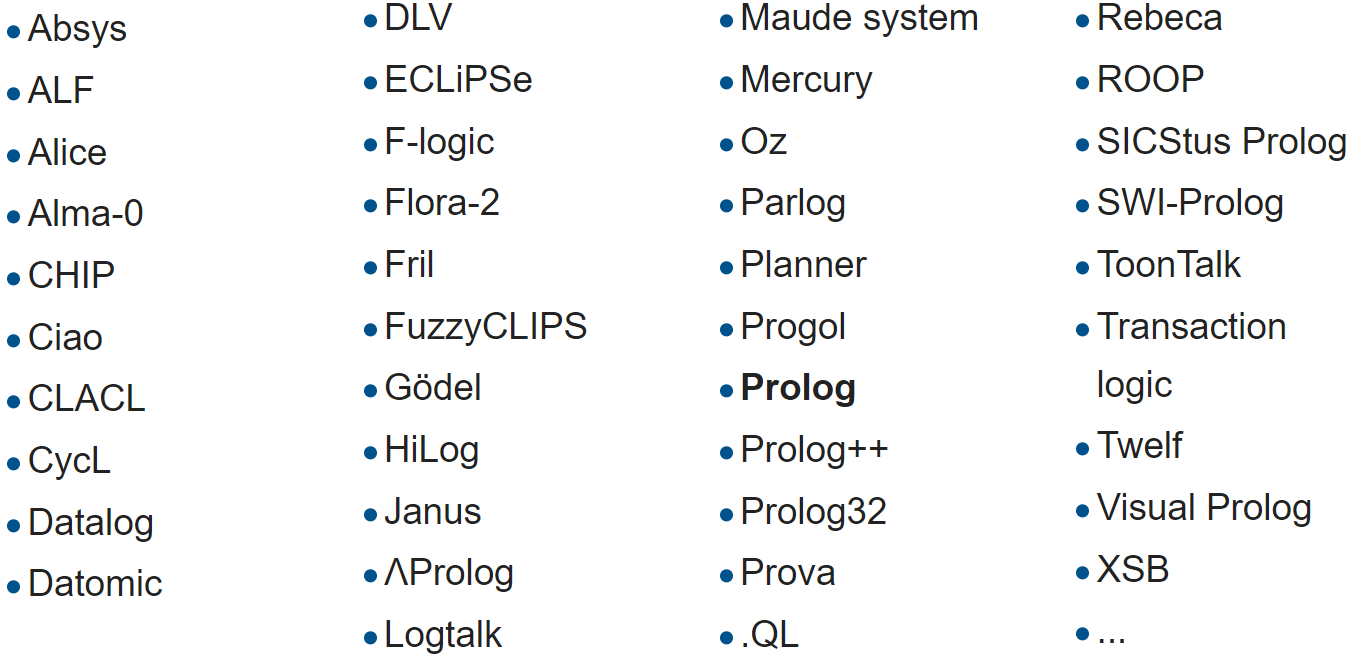
\includegraphics[width=\textwidth]{./image/cap8/lenguajes-logicos.png}
  \end{center}
\end{frame}

%------------------------------
\subsection{Prolog}

\begin{frame}{Prolog}
    \begin{itemize}
        \item Lenguaje creado en 1972 por el francés Alain Colmerauer.
        \item Un programa en Prolog es una base de conocimientos sobre la que se realizan consultas.
    \end{itemize}
    \begin{block}{Ejemplo}
        Sócrates es hombre\\
        Todos los hombres son mortales\\[2ex]
        
        Entonces... \uncover<2->{Sócrates es mortal}
    \end{block}
\end{frame}

\begin{frame}{Prolog}
    \begin{itemize}
        \item<1-> Lo anterior puede representarse así en Prolog:\\[1ex]
    
        \texttt{hombre(socrates). $~~~~~~$} \% un hecho\\
        \texttt{mortal(X):-hombre(X). $~~$} \% una regla
        \item<2-> Los \blue{hechos} son siempre verdaderos y definen por extensión.
        \item<3-> Las \blue{reglas} son implicaciones lógicas y definen por comprensión.
        \begin{itemize}
            \item<4-> La regla anterior significa ``X es hombre $\Rightarrow$ X es mortal''.
            \item<5-> El cuantificador ``para todo'' ($\forall$) está implícito.
            \item<6-> La implicación ($\Rightarrow$) difiere de la lógica tradicional, pues la veracidad del consecuente depende de veracidad del antecedente; si antecedente es falso, no podemos deducir que consecuente sea verdadero.
        \end{itemize}
        \item<7-> Los hechos y las reglas son los dos tipos de \blue{cláusulas}.
        \item<8-> Las constantes van en minúsculas, y variables en mayúsculas.
    \end{itemize}
\end{frame}

\begin{frame}{Principio de universo cerrado}
    \begin{itemize}
        \item<1-> ¿Cómo podemos deducir que Aristóteles también es mortal,\\ i.e., que \blue{\texttt{mortal(aristoteles).}}?
        \item<2-> Así como está la base de conocimientos, NO se puede.
        \item<3-> Falta incluir el hecho: \blue{\texttt{hombre(aristoteles).}}
    \end{itemize}
\end{frame}

\begin{frame}{Más Prolog...}
    \begin{itemize}
        \item Prolog admite conjunciones (Y), disyunciones (O) y negaciones (NO).
        \item Prolog admite ciertas operaciones aritméticas, mediante el predicado \texttt{is}.
        \item Además permite trabajar con \blue{individuos simples} (átomos, números) y \blue{compuestos} (listas, functores).
    \end{itemize}
    \begin{flushright}
        {\small \blue{\url{http://wiki.uqbar.org/wiki/articles/paradigma-logico.html}}}
    \end{flushright}
\end{frame}

\begin{frame}{Ejercicio: Árbol genealógico}
    \begin{itemize}
        \item Considere el árbol genealógico de la Familia Parra:\\ {\small \blue{\url{https://es.wikipedia.org/wiki/Plantilla:Familia_Parra}}}
        \item Definir en Prolog las relaciones familiares directas \blue{padre(Padre,Hijo)} y \blue{madre(Madre,Hijo)}.
        \item Poblar la base del conocimiento y verificar que las relaciones se cumplan.
        \item Definir la relación \blue{progenitor} usando relaciones \blue{padre} y \blue{madre}.
        \item Averiguar cómo se emplea la recursividad en Prolog, y definir recursivamente la relación \blue{antepasado}.
    \end{itemize}
    \begin{flushright}
        \green{[+1 bonus]}
    \end{flushright}
\end{frame}

\begin{frame}{Ejercicio: Red semántica}
    \begin{itemize}
        \item Modele en Prolog la siguiente red semántica:
        
        \begin{center}
          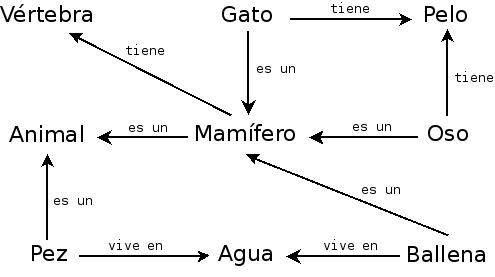
\includegraphics[width=.7\textwidth]{./image/cap8/red-semantica.png}
        \end{center}
        \item Infiera si los gatos son o no animales vertebrados.
    \end{itemize}
    \begin{flushright}
        \green{[+1 bonus]}
    \end{flushright}
\end{frame}

%clase3: Recursivida en lógica:
%http://wiki.uqbar.org/wiki/articles/recursividad-en-logico.html

%clase2: Polimorfismo
%http://wiki.uqbar.org/wiki/articles/polimorfismo-en-el-paradigma-logico.html

% Ejercicios:
% http://www.it.uc3m.es/rcrespo/docencia/irc/lab/Ejercicios_Prolog.pdf
% http://www.cs.us.es/~jalonso/pub/2006-ej_prog_declarativa.pdf

%------------------------------

\begin{frame}
 \begin{block}{Bibliografía}
  \begin{itemize}
    \item Pratt, Terrence W. (1998). \textit{Lenguajes de programación: diseño e implementación}, Pearson Education.
    \item Sethi, Ravi (1992). \textit{Lenguajes de programación: conceptos y constructores}, Addison-Wesley Iberoamericana.
    \item Scott, Michael (2009). \textit{Programming Language Pragmatics}, Morgan Kaufman, 3ra ed.
  \end{itemize}
 \end{block}
 \begin{block}{Recursos}
  \begin{itemize}
    \item Wikipedia y Wikimedia Commons.
    \item Uqbar-wiki: \url{http://wiki.uqbar.org/}
  \end{itemize}
 \end{block}
\end{frame}

\end{document}
